\section{Introduction}
\label{sec:intro}

The research of document understanding has been advanced remarkably in the last decade. However, past works mostly rely on smaller, specialized models, necessitating the design of independent models for each specific task (\eg, document structure parsing). This strategy not only increases the labor in model development but also limits the applicability of the models. Recently, this field has undergone transformation with the rise of large language models (LLMs) and large vision-language models (LVLMs), such as the open-source InternLM-XC2-4KHD~\cite{dong2024internlm} and TextMonkey~\cite{liu2024textmonkey}. These models are showcasing their capabilities in handling complex document elements like charts and images, managing longer contexts up to 128k or more, and tackling diverse tasks in addition to OCR task, such as table question answering and layout understanding.


\begin{figure}
    \centering
    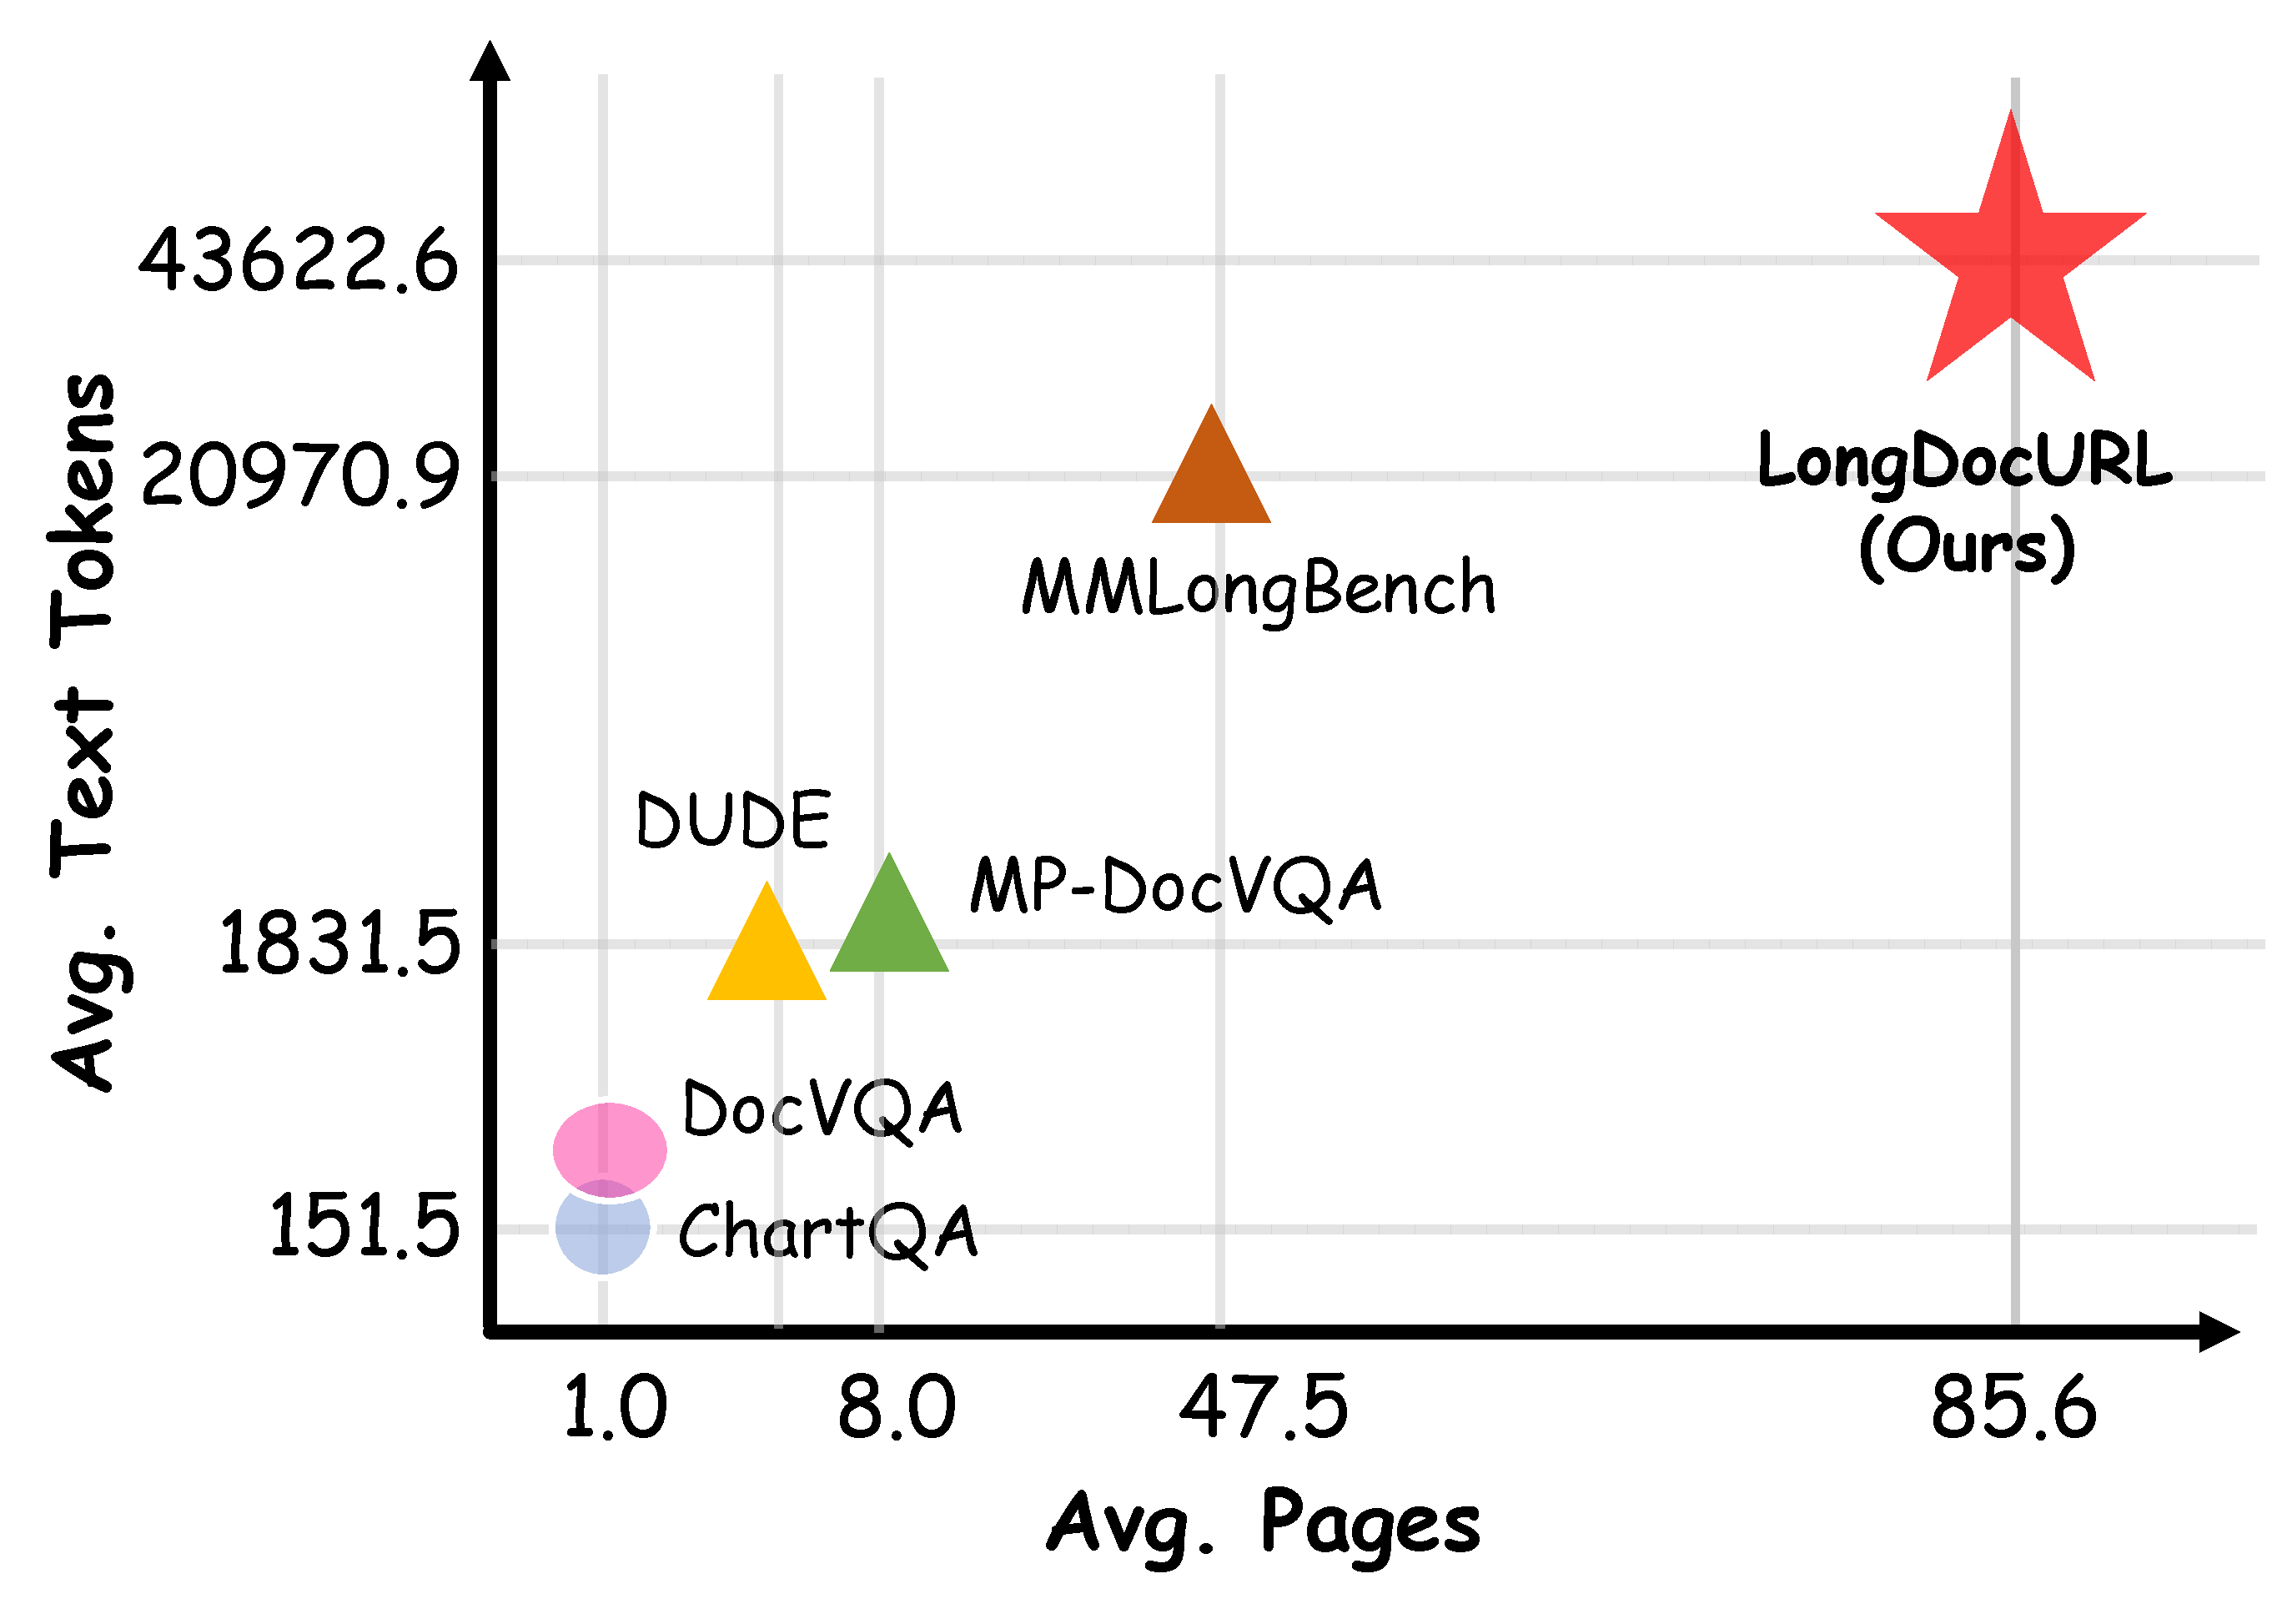
\includegraphics[width=0.5\textwidth]{img/comparison.pdf} 
    \vspace{-0.8cm}
    \caption{Comparison with other datasets in average pages and text tokens per document.}
    \vspace{-0.8cm}
    \label{fig:comparison}
\end{figure}

\begin{figure*}[ht]
    \centering
    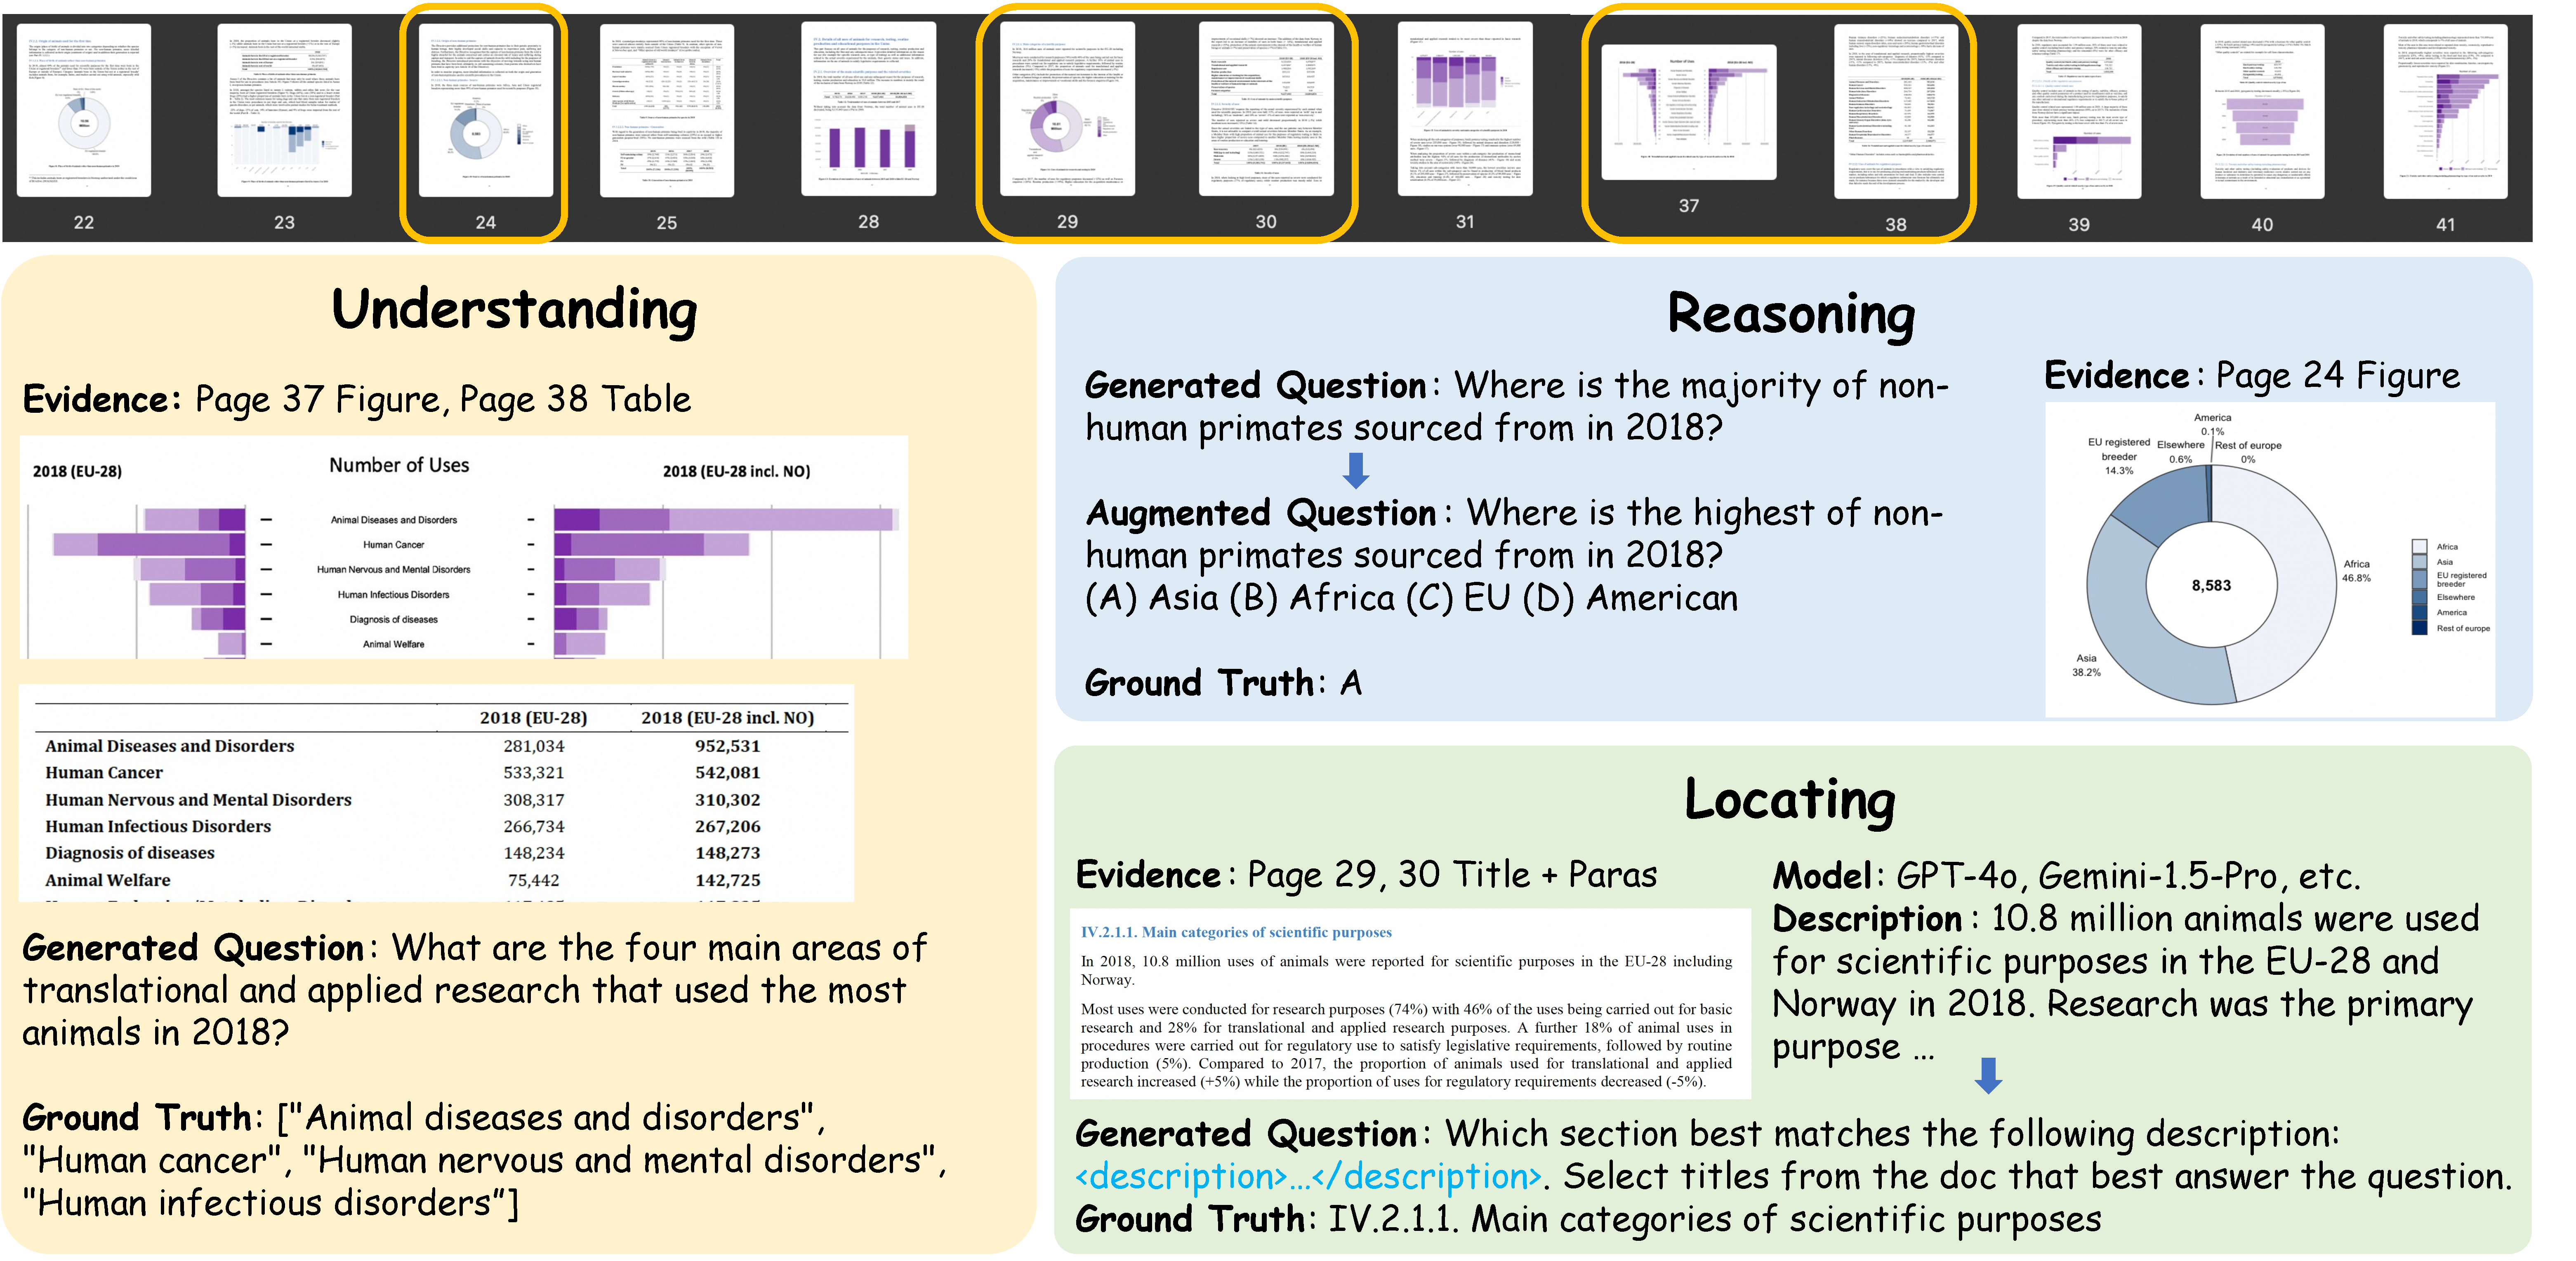
\includegraphics[width=1.0\textwidth]{img/overview_1215.pdf} 
    \vspace{-0.7cm}
    \caption{\benchName~comprises 20 sub-tasks focusing on three task categories: \textbf{U}nderstanding, numerical \textbf{R}easoning, and cross-element \textbf{L}ocating. (Top) Thumbnail of a document example. \textcolor{orange}{Orange} boxes indicate answer evidence pages. (Bottom) Data examples generated from the document and screenshots of relevant part of answer evidence pages.}
    \vspace{-0.5cm}
    \label{fig:overview}
\end{figure*}


Despite the advances in model capabilities, the evaluation of complex document tasks is somewhat lacking. Take DocVQA~\cite{DocVQA} as an example; it is one of the standard benchmarks for document understanding, but it can only assess single-page documents, and many models can easily exceed an accuracy of 95\% (\eg, Qwen2-VL~\cite{Qwen2-VL}). The benchmarks detailed in \Cref{tab:comparison_among_benchmarks} exhibit limitations in adequately addressing complex elements, longer contexts, and diverse tasks: \textbf{1) Complex elements:} Most benchmarks fail to cover all elements such as paragraphs, titles, tables, and figures, focusing instead on only some of the contents. Additionally, discussions about the interrelations among different elements are scarce. \textbf{2) Longer contexts:} Current benchmarks for multi-page document question answering, such as MP-DocVQA~\cite{MP-DocVQA} and DUDE~\cite{DUDE}, do not assess documents exceeding 20 pages. While MMLongBench-Doc~\cite{MMLongBench-Doc} collects longer documents, it offers only approximately 1k effective samples, with only about 30\% of questions involving cross-page information. \textbf{3) Diverse tasks:} Existing work focuses more on OCR or easy question-answering tasks, neglecting the exploration of capabilities in other areas such as cross-element \locating~task (as shown in \Cref{fig:overview}c). The above findings indicate that existing benchmarks lag behind the advances of models, which could hinder the development of document understanding.

\begin{table*}[htbp]
    \centering
    \resizebox{0.95\textwidth}{!}{
    \begin{tabular}{l|cccc|cc|ccc}
        \toprule
        
        \multirow{2}{*}{\textbf{Benchmarks}} & \multicolumn{4}{c|}{\textbf{Data Size}} & \multicolumn{2}{c|}{\textbf{Answer Evidence}} & \multicolumn{3}{c}{\textbf{Task Type}} \\
        
         & \#Docs & \#Avg. Pages & \#Avg. Tokens & \#QA & Multi-page(\%) & Cross-element(\%) & U & R & L \\
        
        \midrule
        
        \multicolumn{2}{l}{\textcolor{gray}{\textit{single-page}}} \\
        DocVQA~\cite{DocVQA} & - & 1.0 & 151.5 & - & \xmark & not specified & \cmark & \xmark & \xmark \\
        ChartQA~\cite{ChartQA} & - & 1.0 &  236.9 & - & \xmark & not specified & \cmark & \xmark & \xmark\\
        
        \multicolumn{2}{l}{\textcolor{gray}{\textit{multi-page(<=20)}}} \\
        MP-DocVQA~\cite{MP-DocVQA} & - & 8.3 & 2,026.6 & - & \xmark & not specified & \cmark & \xmark & \xmark\\
        DUDE~\cite{DUDE} & - & 5.7 & 1,831.5 & - & \cmark(2.1\%) & not specified & \cmark & \cmark & \xmark\\
        
        \multicolumn{2}{l}{\textcolor{gray}{\textit{multi-page(>20)}}} \\
        MMLongBench-Doc~\cite{MMLongBench-Doc} & 135 & 47.5 & 21,214.1 & 1,082 & \cmark(33.0\%) & \cmark(22.6\%) & \cmark & \cmark & \xmark \\
        M-Longdoc~\cite{M-Longdoc-arxiv} & 180 & 210.8 & - & 851 & - & - & \cmark & \cmark & \xmark \\
        
        \midrule
        
        \benchName~(Ours) & 396 & 85.6 & 43,622.6 & 2,325 & \cmark(52.9\%) & \cmark(37.1\%) & \cmark & \cmark & \cmark\\
        \bottomrule
    \end{tabular}}
    \caption{Comparison between \BenchName~and previous document understanding datasets. Task types: (\textbf{U})nderstanding, (\textbf{R})easoning, and (\textbf{L})ocating.}
    \label{tab:comparison_among_benchmarks}
    \vspace{-5mm}
\end{table*}


In this paper, we present a comprehensive document benchmark including three task categories: 1) \textbf{Understanding}: extracting information from documents by identifying keywords, parsing the structure of tables, \etc. Answers are found directly in the document. 2) Numerical \textbf{Reasoning}: processing numerical information through counting, calculating, comparing, and summarizing, requiring both extracted information and reasoning for concluding. 3) Cross-Element \textbf{Locating}: As mentioned earlier, discussions about the interrelations among different types of elements are scarce. It is often necessary to establish a task that evaluates models' ability to analyze relations among different types of elements. For instance, in Para-Title \Locating~task, as shown in \Cref{fig:overview}c, models must summarize relevant sections to identify parts that match a given abstract and then determine the relation between the paragraph and its section titles. This task requires switching element types (\ie, paragraphs to titles) during the answering process.



Our benchmark, named \textbf{\benchName}, comprises 20 sub-tasks according to different primary tasks and answer evidence. More details are presented in \Cref{sec:benchmark}. To efficiently assemble the evaluation dataset for \benchName, we design a semi-automated pipeline comprising four modules. Specifically, a Extract \& Filter module identifies documents of suitable length with rich layouts from diverse document sources. A QA Generation module utilizes a multi-step iterative querying process with advanced models (\eg, GPT-4o) to generate QA pairs with evidence sources. Finally, the Automated Verification and Human Verification modules ensure the quality of the generated content. Through this semi-automated pipeline, we ultimately produce 2,325 QA pairs, covering more than 33,000 pages of documents. Thereafter, we conduct comprehensive evaluation experiments with 26 different configurations (varying the model and input format). These evaluation results indicate that the highest-performing closed-source model, GPT-4o, scored 64.5, leading all models, while the best score for open-source models is only 30.6. This result reveals a potential gap in document understanding and shows the need for further improvement. Our contributions are as follows:
\begin{itemize}[leftmargin=*]
    \item We introduce three primary tasks of long document and propose a comprehensive benchmark comprising 20 sub-tasks categorized based on different primary tasks and answer evidences to support more fine-grained evaluation.
    \item We develop a cost-efficient semi-automated construction pipeline and generate 2,325 high-quality QA pairs, covering more than 33,000 pages of documents, which significantly outperforms existing benchmarks.
    \item We conduct comprehensive evaluation experiments of both open-source and closed-source models under 26 different configurations.
\end{itemize}